\documentclass[a4paper,11pt]{article}

\usepackage{amsmath, amssymb, amstext, amsfonts, mathrsfs}


% \sffamily %schrift ohne Serifen

\usepackage[T1]{fontenc} 
% schriftencodierung f�r umlaute, trennung
% f\"ur Uni
\usepackage[latin1]{inputenc}
\usepackage{selinput}
% \usepackage[utf8x]{inputenc} 
\usepackage{bibgerm} 
% german bibliography
\usepackage[german]{babel}
%wichtig f�r deutschen Content
\usepackage{ucs}
%erweiterte UTF-8 Unterst�tzung
\usepackage{wrapfig} 
% Paket zur Positionierung einbinden
\usepackage{multirow}
% zusammenfassen von Tabellenzellen
% \usepackage{subscript}
% zum tiefstellen
\usepackage{lscape}
\usepackage{pdflscape}
% zum drehen der Seite
% \usepackage[super]{natbib}
\usepackage[square,sort,comma,numbers]{natbib}
% Erstellung es Literaturverzeichnisses
\usepackage{url}
% Umbruch f�r URL
\usepackage{pst-3dplot}
% f�r tex Grafiken n�tig
\usepackage{pstricks}
\usepackage{listings}
% f�r das einf�gen von Quelltext
\definecolor{codegray}{rgb}{0.92,0.92,0.92}
\lstset{basicstyle=\fontsize{9}{11}\selectfont\ttfamily, breaklines=true, backgroundcolor=\color{codegray}, numbers=left, numberstyle=\tiny, tabsize=4, language=java}
\definecolor{mymauve}{rgb}{0.58,0,0.82}
\definecolor{mygreen}{rgb}{0,0.6,0}
\lstset{
commentstyle=\color{mygreen},
keywordstyle=\color{mymauve},
language=Java,
stringstyle=\color{blue}
}


%Einstellungen f�r Quellcode
\usepackage[a4paper, left=3cm, right=2cm, top=2cm]{geometry}
% Formatierung R�nder
\usepackage[section]{placeins}
% f�r Floatbarriere
\usepackage{color}
\usepackage{colortbl}
%f�r die Verwendung von Farben

\clubpenalty = 10000 
\widowpenalty = 10000
\displaywidowpenalty = 10000
%Verhinderung von Hurenkindern und Schusterjungen
%10000 bedeutet die sie sollen kommplett vermieden werden

\title{Entwicklung einer Android-Applikation f�r die Alarmierung der Einsatzkr�fte der Freiwilligen Feuerwehren}

\author{Sebastian Rieger}

\pagenumbering{arabic}
%Seitenzahlen(arabische Zahlen)

\setlength{\parindent}{0.25cm} 
%Absatzeinzug �ndern in Zoll
\setlength{\parskip}{0.25cm}
%Absatzabstand
\linespread {1.5}
%Zeilenabstand

\usepackage{setspace}
\usepackage{hyperref}
%anklickbare Hyperlinks

%funktioniert nicht bei Fu�noten
\usepackage{graphicx}
\usepackage{graphics}
%f�r einbinden von Grafiken

\usepackage{framed}
%f�r Umrandung der Erkl�rung
\usepackage{acronym}
% f�r abk�rzungen
% \usepackage{PSTricks}
\usepackage{epstopdf}
% f�r eps bilder nutze pdflatex --shell-escape this.tex
\usepackage{amssymb}
% f�r mathematische Symbole

\usepackage{hyperref}
% klickbare links

% \usepackage{pdfpages}
\usepackage{rotating}
\usepackage{svg}
%%%%%%%%%%%%%%%%%%%%%%%%%%%%%%%%%%%%%%%%%%%%%%%%%%%%%%%%%%%%%%%%%%%%%%%%%%%%%%%%%%%%%%%%%%%%%%%%%%%%%
%% Angaben zur Arbeit
%%%%%%%%%%%%%%%%%%%%%%%%%%%%%%%%%%%%%%%%%%%%%%%%%%%%%%%%%%%%%%%%%%%%%%%%%%%%%%%

\newcommand{\Autor}{Sebastian Rieger}
\newcommand{\MatrikelNummer}{10286908}
\newcommand{\Kursbezeichnung}{TINF12B1}

\newcommand{\FirmenName}{PDV Systeme}
\newcommand{\FirmenStadt}{Erfurt}
\newcommand{\FirmenLogoDeckblatt}{{
\includegraphics[width=3cm]{Bilder/PDV-Systeme}}}

% Falls es kein Firmenlogo gibt:
%  \newcommand{\FirmenLogoDeckblatt}{}

\newcommand{\BetreuerFirma}{Dipl. -Inform. FH Nico Kaiser}
\newcommand{\BetreuerDHBW}{Prof. Rolf Kruse}
\newcommand{\Titel}{Evaluation moderner Webtechnologien f�r die Entwicklung eines modularen Supportportals}
\newcommand{\AbgabeDatum}{01.03.2017}

\newcommand{\Dauer}{24 Wochen}

% \newcommand{\Abschluss}{Bachelor of Engineering}
\newcommand{\Abschluss}{Master of Science}

\newcommand{\Studiengang}{Angewandte Informatik}
% \newcommand{\Studiengang}{Angewandte Informatik}
\newcommand{\Was}{Master Projekt}

%%%%%%%%%%%%%%%%%%%%%%%%%%%%%%%%%%%%%%%%%%%%%%%%%%%%%%%%%%%%%%%%%%%%%%%%%%%%%%%%%%%%%%%%%%%%%%%%%%%%% 
%steuervariable
\usepackage{ifthen} %Package f�r if/else
\newboolean{bilder} %Deklaration
\setboolean{bilder}{true} %Zuweisung
% \setboolean{bilder}{false} %Zuweisung
%%%%%%%%%%%%%%%%%%%%%%%%%%%%%%%%%%%%%%%%%%%%%%%%%%%%%%%%%%%%%%%%%%%%%%%%%%%%%%%%%%%%%%%%%%%%%%%%%%%%%

\begin{document}

\begin{center}
\vspace*{-2cm}
\FirmenLogoDeckblatt\hfill
\includegraphics[width=4cm]{Bilder/logo_FHE}\\[1cm]
{\Huge \Titel}\\[2cm]
{\Huge\scshape \Was}\\[2cm]
{\large f�r die Pr�fung zum}\\[0.5cm]
{\Large \Abschluss}\\[0.5cm]
{\large des Studienganges \Studiengang}\\[0.5cm]
{\large an der}\\[0.5cm]
{\large Fachhochschule Erfurt}\\[0.5cm]
{\large von}\\[0.5cm]
{\large\bfseries \Autor}\\[1cm]
{\large Abgabedatum \AbgabeDatum}
\vfill
\end{center}
\begin{tabular}{l@{\hspace{1cm}}l}
Bearbeitungszeitraum             & \Dauer                       \\
Matrikelnummer                   & \MatrikelNummer              \\
% Kurs                             & \Kursbezeichnung             \\
Ausbildungsfirma                 & \FirmenName                  \\
                                 & \FirmenStadt                 \\
Betreuer der Ausbildungsfirma    & \BetreuerFirma               \\
Gutachter der Fachhochschule     & \BetreuerDHBW                \\
\end{tabular}

\newpage
%Seitenumbruch
%%%%%%%%%%%%%%%%%%%%%%%%%%%%%%%%%%%%%%%%%%%%%%%%%%%%%%%%%%%%%%%%%%%%%%%%%%%%%%
%% Descr:       Vorlage für Berichte der DHBW-Karlsruhe, Erklärung
%% Author:      Prof. Dr. Jürgen Vollmer, vollmer@dhbw-karlsruhe.de
%% $Id: erklaerung.tex,v 1.2 2010/07/22 13:30:27 vollmer Exp $
%%%%%%%%%%%%%%%%%%%%%%%%%%%%%%%%%%%%%%%%%%%%%%%%%%%%%%%%%%%%%%%%%%%%%%%%%%%%%%%

% In Bachelorarbeiten muss eine schriftliche Erklärung abgegeben werden. In allen anderen
% Arbeiten entf�llt diese. Hierin best�tigen die Studierenden, dass die Bachelorarbeit
% selbst�ndig verfasst und s�mtliche Quellen und Hilfsmittel angegeben sind. Diese Erkl�rung
% bildet das zweite Blatt der Arbeit. Der Text dieser Erkl�rung muss auf einer separaten Seite
% wie unten angegeben lauten.

\newpage
\thispagestyle{empty}
\begin{framed}
\begin{center}
\Large\bfseries Erkl\"arung
\end{center}

\noindent
Ich, \Autor, versichere hiermit, dass ich die vorliegende Masterarbeit mit dem
Thema\\
\hspace*{10mm}\Titel\\
selbstst�ndig und nur unter Verwendung der angegebenen Quellen und Hilfsmittel angefertigt
habe.

\vspace{3cm}
\noindent
\underline{\hspace{4cm}}\hfill\underline{\hspace{6cm}}\\
Ort~~~~~Datum\hfill Unterschrift\hspace{4cm}
\end{framed}

%%%%%%%%%%%%%%%%%%%%%%%%%%%%%%%%%%%%%%%%%%%%%%%%%%%%%%%%%%%%%%%%%%%%%%%%%%%%%%%
\endinput
%%%%%%%%%%%%%%%%%%%%%%%%%%%%%%%%%%%%%%%%%%%%%%%%%%%%%%%%%%%%%%%%%%%%%%%%%%%%%%%

\newpage
\begin{spacing}{0.9}

%Einf�gen Inhaltsverzeichnis
\tableofcontents
\newpage
\section{Einleitung}
In einer vernetzen Welt wie unserer, werden unabl�ssig neue und bessere Web-Technologien entwickelt. Diese neuen Technologien bringen zum einen eine bessere Programmierfreundlichkeit mit sich, aber sie sind zum anderen auch Performanter als fr�here Ans�tze.

Um heute eine Webanwendung zu entwickeln die nicht nur tut was sie soll, sondern die auch performat und auf vielen Systemen l�uft, muss eine Vielzahl von Technoliegen beherrscht und angewendet werden.

Das Ziel diese Arbeit ist es herauszufinden wie neue Technoliegen von heute kombiniert werden k�nnen, um ein m�glichst leistungsstarkes und performantes System zu schaffen.
Hierbei sollen Programmierans�tze wie Google Polymer, AngularJS, HTML5, CSS3, PHP7 und Google Dart under dem Portalserver Typo3 vereint werden.

Es soll gepr�ft werden, wie und ob es m�glich ist diese verschiedenen Technoliegen in m�glichst modularen Typo3-Extensions unterzubringen.

Diese Arbeit soll der theoretischen Grundstock f�r eine weitere Arbeit sein, in der das Support-Portal der PDV System Erfurt GmbH neu entwickelt wird.
Im Verlauf sollen mehrer Beispiel Extensions f�r Typo3 entstehen, welche das Ziel verfolgen Programmierans�tze f�r eine sp�tere Neuentwicklung zu sein.

In den nun folgenden Abschnitten werden Progammierbeispiele und Hinweise gegeben, wie eine solche Neuentwicklung unter den Gesichtspunkten Performance, Umsetzbarkeit und Usability vorgenommen werden kann.
\newpage
\section{Portalserver/ CMS-Systeme im Vergleich}
Das zuk�nftige Supportportal der PDV Systeme GmbH soll auf Basis eines Portalservers bzw. \ac{CMS}-Servers aufgebaut werden. Hierf�r werden im folgenden einige M�glichkeiten genauer betrachtet.

Ein Portalserver, welcher f�r das Projekt heran gezogen wird muss die folgenden Eigenschaften aufweisen.
\begin{itemize}
 \item Webseiten m�ssen frei gestalltbar sein
 \item Es muss die M�glichkeit bestehen Anwendungen f�r den Server zu entwickeln
 \item Das System muss Open-Source sein, um ggf. in den Quellcode eingreifen zu k�nnen
 \item Die Nutzer-Community sollte m�glichst gro� sein, damit Probleme leicht diskutiert und behoben werden k�nnen
 \item Der Server muss die M�glichkeit bieten Dateien zu verwalten, welche als Download oder Kontent in das Portal einflie�en
 \item Lauff�hing unter einer SQL-Datenbank wie MySQL oder MariaDB
\end{itemize}

Auf die Betrachtung reiner \ac{CMS}-System wird an dieser Stelle verzichtet, da diese nicht die gew�nschten Anforderungen eines Portalservers erf�llen.
Ein Vergleich verschiedener reiner \ac{CMS}-Systeme ist in der Bachelorarbeit "`Konzept und prototypische Implementierung eines �bergreifenden Dokumenten- und Medienmanagements"' zu finden.
\cite{Bachelorarbeit}


\subsection{Typo3}\label{PortalServerTypo3}
Typo3 ist ein Verwaltungssystem f�r Internetseiten. Es basiert in der neusten Version 8.2 auf der PHP Version 7. 
Seit der Version 7.0 welche zugleich eine \ac{LTS} Version ist, wird es unter dem Namen Typo3 \ac{CMS} vertrieben. 
\cite{WikiTypo3}

\begin{figure}[!ht]
\centering
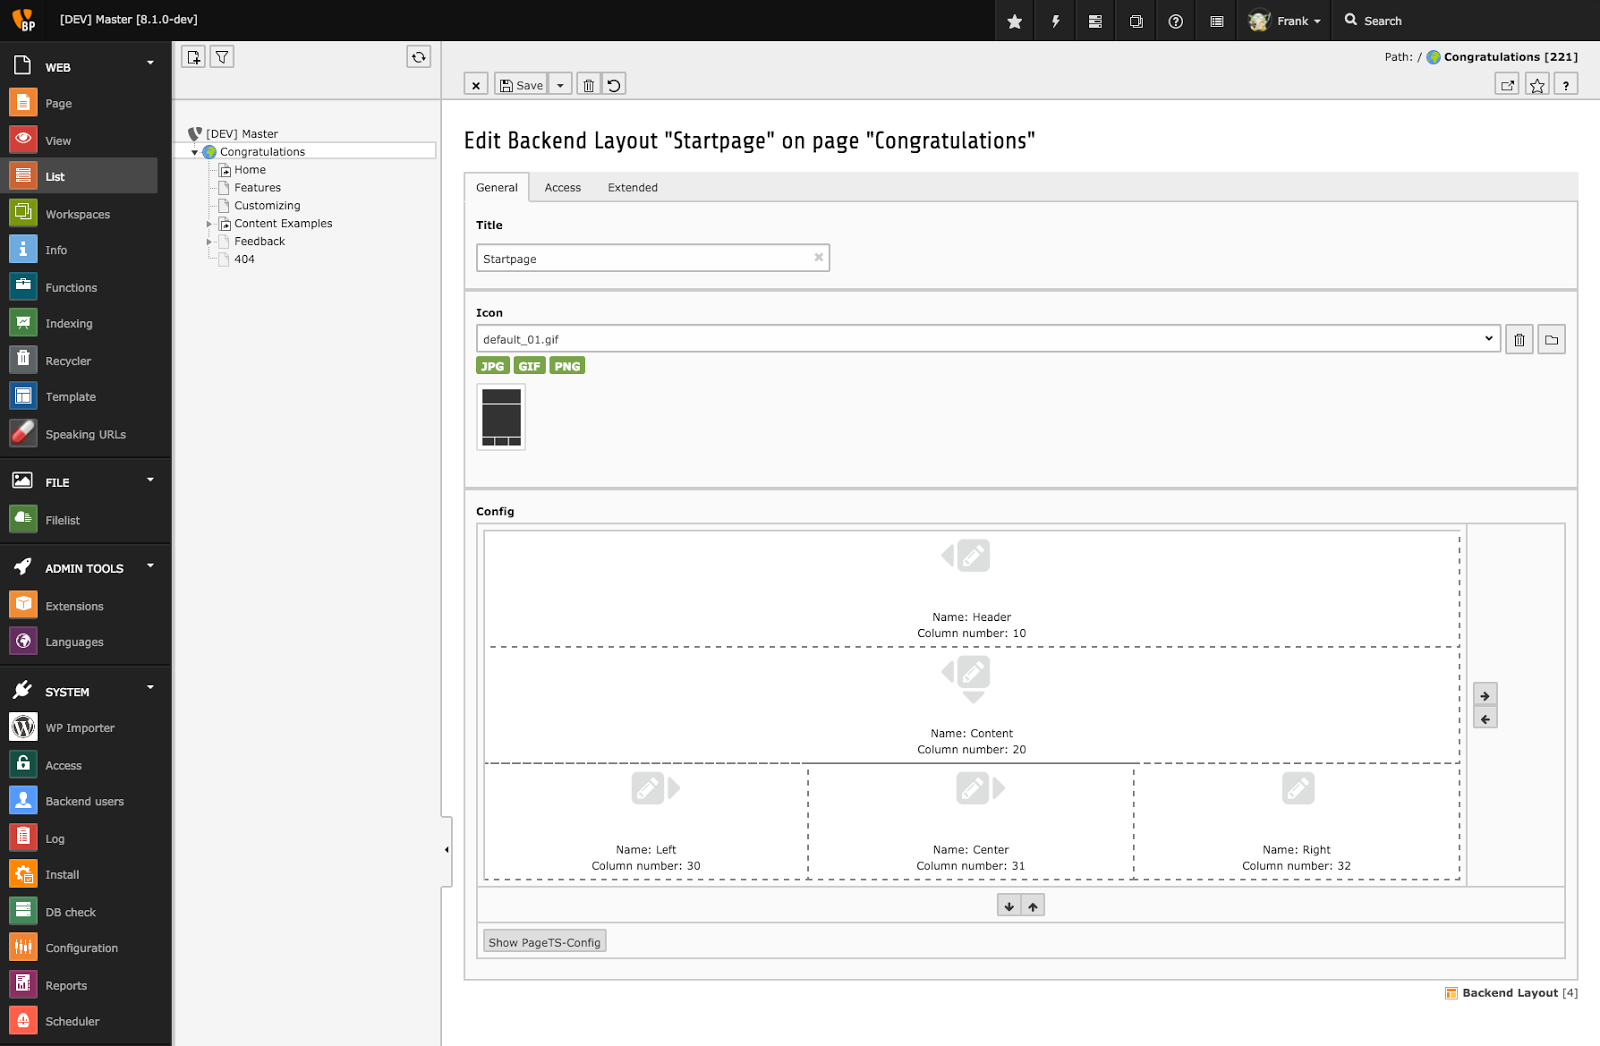
\includegraphics[width=16cm]{Bilder/Typo3_Backend.png}
\caption{Typo3 Backend im Seitenbearbeitungs Modus \cite{Typo3Bild}}
\label{Typo3_Backend_Bild}
\centering
\end{figure}

Es ist m�glich unter Verwendung von PHP, Extbase und Fluid eigene Erweiterungen f�r den Portalserver zu entwickeln. Die jeweiligen Erweiterungen wirken im Fronten von Typo3 wie ganz normale Webseiten.
Auf Extbase und Fluid wird im Kapitel \ref{Typo3} genauer eingegangen.

Ein Vorteil von Typo3 ist, dass es eines der am h�ufigsten verbreiteten Portalserver auf dem Markt ist. Selbst gro�e Firmen wie "`Sixt"' setzten auf Typo3 bei der Erstellung ihrer Internetportale.
Durch die gro�e Verbreitung von Typo3 ist auch die Community um die Software sehr gro� und man findest schell zu fast jedem Problem im Internet eine L�sung.

Typo3 kann im Zusammenspiel mit MySQL, MariaDB, PostgreSQL oder Oracle als Datenbank betrieben werden. Nur mit Hilfe einer dieser Datenbank im Hintergrund ist Typo3 stabil Lauff�hing und kann produktiv eingesetzt werden.

Durch ein �bersichtliches Backend (siehe Abbildung \ref{Typo3_Backend_Bild}), ist es auf f�r Laien m�glich qualitativ Hochwertige Webseiten zu erstellen, ohne viel Kenntnis von Webtechnologien wie HTML oder CSS zu haben.

Ein Upload von Dateien f�r den Download beziehungsweise als Seiten-Kontent ist ebenfalls unter Typo3 m�glich. Zus�tzlich dazu ist es m�glich das Nutzer Dateien auf den hochladen. 
Hierdurch entsteht auch die M�glichkeit ein Austauschportal f�r Dateien zu schaffen. Nutzer k�nnen so in einer sicheren Umgebung sensible Daten untereinander oder mit Mitarbeitern austauschen.
\cite{LobacherTypo3}

\subsection{Typo3 Neos}
Typo3 Neos ist ein relativ neuer Internetportal Server, welcher 2012 aus dem Wunsch heraus entstand Typo3 zukunftssicher zu gestalten.

Als erkannt wurde, dass eine zukunftssichere Typo3 Entwickung basierend auf dem \ac{MVC}-Prinzip eine koplette Neuimplementierung erfordert wurde der Grundstein f�r Typo3 Neos gelegt.
Neben der Entwickung von Typo3 \ac{CMS} wurde die Entwicklung von Typo3 Neos begonnen. Das Ziel war es, einen Nachfolger f�r Typo3 zu entwickeln. Dies gelang jedoch nicht wie vorgesehen.
\cite{WikiTypo3}

Fr�h wurde festgestellt das sich diese die beiden Projekte in unterschiedliche Richtungen entwickeln. Typo3 Neos ist heute in der Version 2.0 erh�ltlich und hat sich zum Ziel gesetzt Webseiten im gegensatz zu Typo3 live im Frontend zu bearbeiten.
Einfach gesagt ist Typo3 ein Internet-Portalserver welcher auf dem \ac{WYSIWYG}-Prinzip aufbaut. Es ist m�glich Webseiten live oder getrennt vom Livesystem im Frontend zu erstellen. 
Die Frontend-Bearbeitung bingt viele Vorteile f�r die Webseitenerstellung f�r Laien. Diese k�nnen eine Seite direkt bearbeiten und Live nehmen.
\cite{LobacherTypo3}

Neos ist bei weitem nicht so verbreitet wie Typo3 \ac{CMS} und die Community um das Projekt ist deutlich geringer. Dies ist ein klarer Nachteil zum gro�en Bruder Typo3 \ac{CMS} ist.

�hnlich wie bei Typo3 \ac{CMS} ist es in Neos m�glich sogenannte Plugins zu entwickeln. Diese basieren auf dem "`Typo3 Flow"'-Framework, welche zusammen mit Neos entwickelt wurde.
Flow ist ein Framework, welches es erlaubt Templates mit Hilfe von "`Fluid"' zu entwickeln. Auf die Fluid wird im Abschnitt \ref{Fluid} n�her eingegangen.
\cite{WikiFlow}

�hnlich wie Typo3 \ac{CMS} ben�tigt auch Neos eine SQL-Datenbank zur Datenhaltung und ist Quelloffen verf�gbar. Nach der Abspaltung von Typo3 Neos vom Typo3 Projekt, wird es heute von einer relativ kleinen Gemeinde entwickelt.
Aus diesem Grund, gibt es keine Roadmap f�r das Projekt und die Ver�ffentlichung von neuen Version ist tr�ger als die von Typo3 \ac{CMS}. 

\begin{figure}[!ht]
\centering
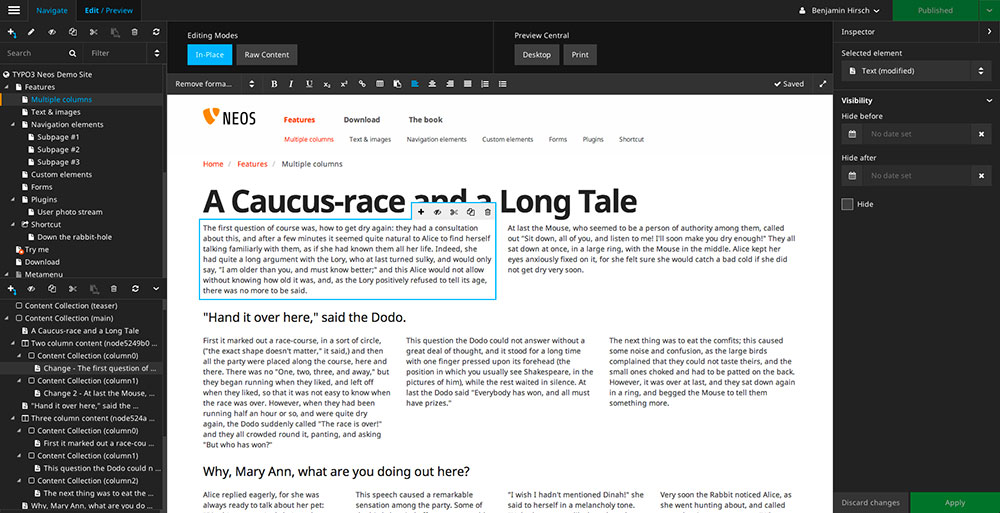
\includegraphics[width=16cm]{Bilder/neos_backend.jpg}
\caption{Typo3 Neos Backend im Seitenbearbeitungs Modus \cite{NeosBild}}
\label{Typo3_Neos_Backend_Bild}
\centering
\end{figure}

In Abbildung \ref{Typo3_Neos_Backend_Bild} ist der Seitenbearbeitungs-Modus von Neos zu sehen. Es ist gut zu erkennen, das Inhalte einer Webseite direkt bearbeitet werden k�nnen. Dies macht eine Webentwicklung f�r Laien einfacher.
\subsection{Joomla}
Joomla ist ein weiteres \ac{CMS}-System f�r die Erstellung von Webseiten. �hnlich wie Typo3 ist es Open Source und nutzt eine MySQL-Datenbank im Hintergrund. Das System ist in PHP5 geschrieben und dient in erster Linie zur Erstellung von Webseiten.
Am besten kann Joomla mit Typo3 Neos verglichen werden, da es einen �hnlichen Ansatz zur Erstellung von Webseiten aufgreift. 

Ein Vorteil gegen�ber Neos ist, das Joomla weit verbreitet ist und eine beachtliche Community hat, welche bei Neos geringer ausf�llt. Nachteilig an Neos ist jedoch, das es eine Bearbeitung von Web-Inhalten nur im Backend zul�sst. Dies bedeutet wiederum, das mehr Erfahrung ben�tigt wird um eine Webseite zu erstellen.

Weitere Nachteile sind zum einen die kaum existente Roadmap, welche zur Zeit der Bearbeitung nicht aktuell war. Zum anderen ist die Entwicklung von Erweiterungen f�r Joomla nicht so gut strukturiert wie es bei Typo3 mit Fluid der Fall ist.

Eine freie Gestalltung der Webseiten ist zwar gegeben, aber f�r die Entwicklung eines komplexes Supportportals wie es sp�ter einmal entstehen soll ist Joomla nicht oder nur bedingt geeignet.
Es gibt momentan keine garantierte Weiterentwicklung des Portalservers und eine Unterst�tzung von MariaDB ist nicht offiziell gegeben.

Auch wenn Joomla durchaus seinen Charm hat, so ist es f�r die Entwicklung eines Supportportals, welches modular aufgebaut werden soll nicht zu empfehlen. Dies bedingt sich zum einen aus der abgelaufen Roadmap, aber auch durch die schlechtere Erweiterungsentwicklung im Gegensatz zu Typo3 \ac{CMS} oder Neos.
\subsection{Drupal}
\subsection{Auswertung der m�glichkeiten}
Auch wenn Typo3 Neos Typo3 \ac{CMS} in nichts nachsteht, so wurde sich dennoch gegen die Verwendung von Neos entschieden, da eine vorranscchreitende Entwicklung nicht gewehrleistet. 
Im Punkto Zukunftssicherheit ist Typo3 \ac{CMS} deutlich besser aufgestellt. 



\end{spacing}




\newpage
\section{Abk�rzungsverzeichnis}
\begin{acronym}
%   \acro{}{\emph{}}
 \acro{CMS}{\emph{Content Managemente System}}
\acro{LTS}{\emph{Long Term Support}}
\acro{MVC}{\emph{Model View Controller}}
\acro{WYSIWYG}{\emph{What you see is what what you get}}
\acro{CSS}{\emph{Cascading Style Sheets}}
\acro{SASS}{\emph{Syntactically Awesome Stylesheets}}
\acro{MVVM}{\emph{Model View ViewModel}}
\acro{RTE}{\emph{Real Time Editor}}
 %  \acro{GDS}{\emph{Generic Data Services}}
% %  \acro{LSDF}{\emph{Large Scale Data Facility}}
%  \acro{OPM}{\emph{Objektorientierten Programmiermodell}}
%  \acro{SMD}{\emph{Strukturelle Metadaten}}
%  \acro{JSON}{\emph{JavaScript Object Notation}}
% %  \acro{HALO}{\emph{High Altitude and Long Range Research Aircraft}}
%  \acro{IAI}{\emph{Institut f�r Angewandte Informatik}}
%  \acro{JAXB}{\emph{Java Architecture for XML Binding}}
%  \acro{UDDE}{\emph{User Data Description Editor}}
%  \acro{AMD}{\emph{Anwendermetadaten}}
%  \acro{CG}{\emph{Class Generator}}
%  \acro{IG}{\emph{Interface Generator}}
\end{acronym}
\newpage
\listoffigures
\newpage
\listoftables
% Abk�rzungsverzeichnis
\newpage
\bibliographystyle{alpha}
% verzeichnis im DIN format
\bibliography{Quellen}
\end{document}
